\chapter{Συνδεσμολογία}

\subsection{Μικροελεγκτής AVR}

Σύμφωνα με τον \textcite[1]{myklebust97}, οι μικροελεγκτές AVR διαθέτουν
μειωμένο σύνολο εντολών, δηλαδή είναι υπολογιστές RISC (\te{Reduced Instruction
Set Computer}). Το χαρακτηριστικό αυτό απλοποιεί τα απαιτούμενα κυκλώματα
ελέγχου και τους παρέχουν μικρότερους κύκλους για την εκτέλεση κάθε εντολής
\parencite[1]{sequin82}. Επιπροσθέτως, οι μικροελεγκτές AVR βασίζονται σε
τροποποιημένη αρχιτεκτονική Harvard σύμφωνα με την οποία, και σε αντίθεση με την
κατά Von Neumann αρχιτεκτονική, το πρόγραμμα και τα δεδομένα τοποθετούνται σε
ανεξάρτητα φυσικά μέσα που χαρακτηρίζονται, μεταξύ άλλων, από ανεξάρτητους
διαύλους πρόσβασης \parencite[1]{myklebust97}.

Άμεσα πλεονεκτήματα αυτού του σχεδιασμού είναι ότι καθίσταται δυνατή η
ταυτόχρονη πρόσβαση στις μνήμες προγράμματος και δεδομένων στον ίδιο κύκλο
\parencite[8]{atmel13}. Επιπλέον, επιτρέπεται η χρήση διαφορετικών τεχνολογιών
για κάθε μνήμη. Για παράδειγμα, στην περίπτωση του χρησιμοποιούμενου
μικροελεγκτή, ATmega328, τα δεδομένα οργανώνονται σε μνήμη πλάτους των 8bit
τεχνολογίας SRAM (\te{Static RAM}) με 2KiB συνολική χωρητικότητα, ενώ οι
εντολές, σε μνήμη Flash των 32KiB με θέσεις των 16bit
\parencite[8--9,16,18]{atmel13}.


Κατά την εκκίνηση της συσκευής, δηλαδή κατά τη σύνδεσή της με την παροχή
τροφοδοσίας, εκτελείται η αρχικοποίηση των διαφόρων υποσυστημάτων της υλοποίησης
και, εν συνεχεία, ο μικροελεγκτής μεταπίπτει σε κατάσταση χαμηλής κατανάλωσης
ισχύος. Από αυτήν, ενεργοποιείται αυτόματα είτε για την εκκίνηση ενός νέου
κύκλου μετρήσεων (βλ. \nameref{sec:task} σ.~\pageref{sec:task}), είτε για την
εξυπηρέτηση κάποιου εισερχόμενου αιτήματος HTTP (βλ. \nameref{%
sec:network:impl-resources} σ.~\pageref{sec:network:impl-resources}). Στο σχήμα
\ref{fig:mcu:tasks} παρουσιάζεται ο κύκλος καθηκόντων του μικροελεγκτή.

\begin{figure}
    \caption{Καθήκοντα του μικροελεγκτή.\label{fig:mcu:tasks}}
    \begin{center}
    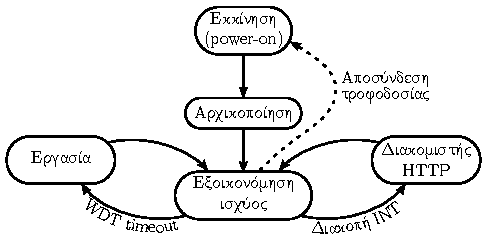
\includegraphics{mcu_tasks}
    \end{center}
\end{figure}

Αναλυτικότερα, κατά το στάδιο της αρχικοποίησης, τίθεται η συχνότητα του
ρολογιού του μικροελεκτή, η οποία, για τις ανάγκες της υλοποίησης, μειώνεται από
τα 16MHz στα 4MHz και η κατεύθυνση των ακροδεκτών (δηλαδή ποιοι είναι εισόδου
και ποιοι εξόδου). Επίσης, ρυθμίζεται το κύκλωμα WDT (\te{Watch-Dog Timer}), το
οποίο είναι υπεύθυνο για την περιοδική αφύπνιση του μικροελεγκτή ώστε να
ελέγχεται η ανάγκη εκκίνησης νέου κύκλου μετρήσεων.

Επιπλέον, ανακτώνται οι μεταβλητές ρυθμίσεις της συσκευής είτε από τις
προκαθορισμένες (εργοστασιακές ρυθμίσεις), είτε από τις αποθηκευμένες τιμές της
εφεδρικής μνήμης, εφόσον αυτές είναι έγκυρες (βλ \nameref{subsec:backup-memory}
σ.~\pageref{subsec:backup-memory}).
Οι ρυθμίσεις αυτές περιλαμβάνουν τη δικτύωση της συσκευής (διεύθυνση IP, μάσκα
υποδικτύου, προεπιλεγμένη πύλη), το λειτουργικό εύρος του υποσυστήματος κίνησης
(βλ. \nameref{sec:motor:coordinates} σ.~\pageref{sec:motor:coordinates}), το
χρονικό διάστημα μεταξύ κύκλων εργασίας καθώς και το πλήθος μετρήσεων που
πραγματοποιείται σε κάθε κύκλο (βλ. \nameref{sec:task} σ.~\pageref{sec:task}).
Ο τρόπος ρύθμισης της συσκευής περιγράφεται στους Πόρους υλοποίησης (σ.~%
\pageref{sec:network:impl-resources}).

Στην πορεία, οι ρυθμίσεις προωθούνται στις κατάλληλες μονάδες και εκτελούνται
επιπρόσθετες προετοιμασίες, όπως η παλιννόστηση της κεφαλής, δηλαδή η επαναφορά
της στη θέση επιστροφής (συντεταγμένες [0, 0, Z\tsub{max}]) (βλ. σ.~%
\pageref{sec:motor:homing}) και η αρχικοποίηση του HTTP \te{Socket} (βλ. σ.~%
\pageref{ssubsec:network:port_mr}).


\subsection{Κατάσταση χαμηλής κατανάλωσης}

Ο μικροελεγκτής διαθέτει διαφορετικές καταστάσεις νάρκης (\te{sleep mode}
όπου η καθεμία απενεργοποιεί ορισμένα κυκλώματα για τη μείωση της κατανάλωσης.
Για παράδειγμα, η πιο απλή, είναι η κατάσταση αδράνειας (\te{idle}) κατά την
οποία απενεργοποιείται μόνο το ρολόι της CPU και της μνήμης Flash (δηλαδή, της
μνήμης προγράμματος). Στο πλαίσιο της υλοποίησης, γίνεται προσπάθεια για την
ύψιστη μείωση της κατανάλωσης κατά τα διαστήματα όπου ο μικροελεγκτής παραμένει
άεργος.

Για το σκοπό αυτό, εφαρμόζεται η κατάσταση \te{power-down} κατά την οποία
απενεργοποιούνται όλα τα ρολόγια του μικροελεγκτή (clk\tsub{CPU}, clk%
\tsub{FLASH}, clk\tsub{IO}, clk\tsub{ADC}, clk\tsub{ASY}) καθώς και οι
ταλαντωτές του συστήματος και των Χρονομετρητών\slash{}Απαριθμητών \parencite%
[38]{atmel13}. Σύμφωνα με την \textcite[38]{atmel13}, ο μικροελεγκτής είναι
δυνατό να επανέλθει σε κανονική λειτουργία μόνο μέσω των ακροδεκτών INT1:0 με
παρατεταμένο λογικό 0 (\te{low-level interrupt}) καθώς και μέσω των κυκλωμάτων
TWI (\te{Two-Wire Interface}) και WDT (\te{Watch-Dog Timer}).

Στο πλαίσιο της υλοποίησης χρησιμοποιείται ο πρώτος και ο τελευταίος τρόπος· το
κύκλωμα TWI αφυπνίζει το μικροελεγκτή όταν αυτός ρυθμίζεται με ρόλο \te{slave}
στο δίαυλο TWI και κάποιο εξωτερικό κύκλωμα προσπαθεί να επικοινωνήσει μαζί του
ενώ, στην υλοποίηση, χρησιμοποιείται μόνο ως \te{master} για την επικοινωνία με
το ρολόι πραγματικού χρόνου (RTC) (βλ. \nameref{sec:rtc} σ.~\pageref{sec:rtc}).

Για την ακρίβεια, ο ένας εκ των δύο ακροδεκτών INT1:0 συνδέεται με τον ακροδέκτη
\nbar{INT} του ολοκληρωμένου δικτύωσης, W5100, το οποίο τον θέτει και τον
διατηρεί σε λογικό 0 έως ότου διευθετηθούν όλες οι ενδείξεις διακοπών που του
έχουν ενεργοποιηθεί
(βλ. \nameref{subsec:network:interface} σ.~\pageref{subsec:network:interface}).
Για τις ανάγκες της υλοποίησης, αυτό σημαίνει ότι έχει καταφθάσει εισερχόμενο
αίτημα HTTP το οποίο διεκπεραιώνεται από το διακομιστή (βλ.
\nameref{sec:http-server} σ.~\pageref{sec:http-server}).

Ο χρονομετρητής WDT ρυθμίζεται ώστε να αφυπνίζει το μικροελεγκτή κάθε 8s (το
μέγιστο διάστημα που υποστηρίζεται από τον παρόντα μικροελεγκτή) και αποτελεί το
έναυσμα για την εκκίνηση νέου κύκλου εργασιών
(\nameref{ssubsec:task:initiate} σ.~\pageref{ssubsec:task:initiate}).







